  \let\negmedspace\undefined
\let\negthickspace\undefined
\documentclass[journal]{IEEEtran}
\usepackage[a5paper, margin=10mm, onecolumn]{geometry}
\usepackage{lmodern} % Ensure lmodern is loaded for pdflatex
\usepackage{tfrupee} % Include tfrupee package

\setlength{\headheight}{1cm} % Set the height of the header box
\setlength{\headsep}{0mm}     % Set the distance between the header box and the top of the text

\usepackage{gvv-book}
\usepackage{gvv}
\usepackage{cite}
\usepackage{amsmath,amssymb,amsfonts,amsthm}
\usepackage{algorithmic}
\usepackage{graphicx}
\usepackage{textcomp}
\usepackage{xcolor}
\usepackage{txfonts}
\usepackage{listings}
\usepackage{enumitem}
\usepackage{mathtools}
\usepackage{gensymb}
\usepackage{comment}
\usepackage[breaklinks=true]{hyperref}
\usepackage{tkz-euclide} 
\usepackage{listings}                                      
\def\inputGnumericTable{}                                 
\usepackage[latin1]{inputenc}                                
\usepackage{color}                                            
\usepackage{array}                                            
\usepackage{longtable}
\usepackage{multicol}
\usepackage{calc}                                             
\usepackage{multirow}                                         
\usepackage{hhline}                                           
\usepackage{ifthen}                                           
\usepackage{lscape}
\begin{document}
	
	\bibliographystyle{IEEEtran}
	\vspace{3cm}
	
	\title{8.2.5}
	\author{EE24BTECH11059 - Y Siddhanth}
	% \maketitle
	% \newpage
	% \bigskip
	{\let\newpage\relax\maketitle}
	
	\renewcommand{\thefigure}{\theenumi}
	\renewcommand{\thetable}{\theenumi}
	\setlength{\intextsep}{10pt} % Space between text and floats
	
	
	\numberwithin{equation}{enumi}
	\numberwithin{figure}{enumi}
	\renewcommand{\thetable}{\theenumi}
	
	
	\textbf{Question}:\newline
	Using integration, find the area of the triangular region whose sides have the equations \(y = 2x + 1\), \(y = 3x + 1\), and \(x = 4\).
	
	\textbf{Solution: }\\
	Theoretical Solution: \\
	First, we find the intersection points, clearly x = 4 is the intersection point for 2 sides.	
	\begin{align}
		-3x + y &= 1 \\ 
		-2x + y &= 1
	\end{align}
	Taking an augmented matrix to solve the above equations,
	\begin{align}
		\myvec{-3 & 1 & 1 \\ -2 & 1 & 1 }
	\end{align}
	
	Using row operations to reduce it,
	\begin{align}
			\myvec{-3 & 1 & 1 \\ -2 & 1 & 1 } \xrightarrow[R_2 \rightarrow R_2 - \frac{2}{3}R_1]{} \myvec{ -3 & 1 & 1 \\ 0 & \frac{1}{3} & \frac{1}{3} } \xrightarrow[R_1 \rightarrow -\frac{1}{3}R_1]{R_2 \rightarrow 3R_2} \myvec{ 1 & -\frac{1}{3} & -\frac{1}{3} \\ 0 & 1 & 1} \xrightarrow{R_1 \rightarrow R_1 + \frac{1}{3}R_2} \myvec{1 & 0 & 0 \\ 0 & 1 & 1}
	\end{align}
	
	Thus, the intersection of the lines $\brak{-3x + y = 1  , -2x + y = 1}$ is $\brak{0,1}$\\
	To find the area, we integrate the difference between the two lines from their intersection point at $x=0$ to $x=4$:
	
	\begin{align}
	Area &= \int_0^4 ((3x+1) - (2x+1)) dx \\ &=\int_0^4 x dx \\&= \left[ \frac{1}{2}x^2 \right]_0^4 \\&= \frac{1}{2}(4^2) - \frac{1}{2}(0^2) \\&= 8
	\end{align}
	
	Thus, the area of the triangular region is 8 square units.

	Numerical Solution:\newline
	The numerical solution for this question can be found using the trapezoidal rule \eqref{trap}.
	\begin{align}
		A  = \int_a^b f(x) \, dx \approx \frac{h}{2} \left[ f(a) + 2f(x_1) + 2f(x_2) + \dots + 2f(x_{n-1}) + f(b) \right]
		\label{trap}
	\end{align}
	Here, $h = \frac{b-a}{n}$, and $n$ is the number of nodes where $x_j$ and $a,b$ are called nodes.
	\begin{align}
		f\brak{x} &= (3x+1) - (2x+1) = x\\
		A &= \int_a^b x \, dx \\ &\approx \frac{h}{2} \left[ a + 2x_1 + 2x_2 + \dots + 2x_{n-1} + b \right]
	\end{align}
	Clearly, $a, x_j, b $ are in an A.P, where $x_i = a+ih$. Thus,
	\begin{align}
		A &\approx \frac{h}{2} \left[ a + \brak{2a+ h} + \brak{2a + 4h} + \dots + \brak{2a + 2(n-1)h} + \brak{a + nh} \right] \\
		&\approx \frac{h}{2} \left[ 2na + (n-1)nh \right]
	\end{align}
	Apply definition of $h$ and values of $a,b$ to the above equation, we get
	\begin{align}
		A &\approx \frac{4}{2n} \left[ 2n(0) + (n-1)(4) \right]\\
		A&\approx \frac{8(n-1)}{n}
	\end{align} 
	Clearly, as n gets larger or the number of nodes increase, the value of area approaches the theoretical value. Taking n as 100000,
			\begin{align}
				A &\approx 7.99992 \\ A &\approx 8
			\end{align} 
	\begin{figure}[h!]
		\centering
		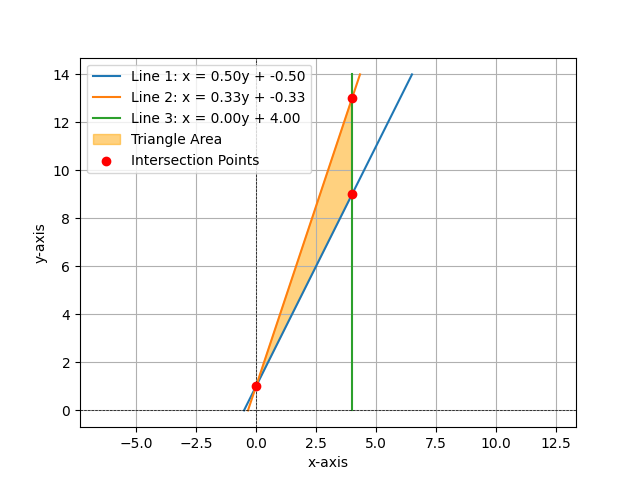
\includegraphics[width=\columnwidth]{figs/fig1.png}
		\caption{Comparison between the Theoretical solution and Numerical solution}
		\label{stemplot}
	\end{figure}
\end{document}  